\section{Experimentos y Resultados}
% Para la experimentación realizada en este trabajo decidimos comenzar implementando la estrategia \textbf{Grid search},
% la cual nos permitio encontrar la mejor configuracion de hiperparametros entre un subconjunto creado por nosotros. Estos
% hiperparametros son: \textit{learning rate} y \textit{discount} para el algoritmo de \textbf{QLearning}, y el epsilon para
% la politica de control \textbf{$\epsilon-greedy$}. La busqueda fue realizada entre los siguientes valores de cada uno:
%
% \begin{itemize}
%   \item  \textbf{$\epsilon$} = 0.1, 0,2
%   \item \textbf{learning\_rate} = 0.1, 0.2, 0.4, 0.6, 0.8, 0.9, 1.0
%   \item \textbf{discount} = 0.5, 0.6, 0.7, 0.8, 0.9
% \end{itemize}
%
%
% Obteniendo como mejor resultado la siguiente configuracion:
%
% \begin{itemize}
%   \item  \textbf{$\epsilon$} = 0.1
%   \item \textbf{learning\_rate} = 0.4
%   \item \textbf{discount} = 0.9
% \end{itemize}
%
% Ademas de estos hiperparametros para el algoritmo y la politica elegida, tambien necesitamos una cantidad de epocas para
% entrenar y un oponente contra quien jugar.
% Así que tomamos algunas decisiones:

\todo{AGREGAR SECCION CON INSTRUCCIONES PARA CORRER LAS COSAS}

Para entrenar al agente que jugará al 4 en línea utilizamos el algoritmo \textbf{QLearning}. Este algoritmo utiliza los hiperparámetros \textit{learning rate} y \textit{discount} y los valores de inicialización de la matriz de Q. Además de estos hiperparámetros, necesitamos una política de control, una cantidad de épocas para entrenar y un oponente contra quien jugar.  \\

Tratar todas las combinaciones no es posible computacionalmente, es por esto que tomamos algunas decisiones sobre los parámetros a utilizar, que se irán modificando en base a la experimentación realizada:

\begin{enumerate}
\item La cantidad de epocas para entrenar serán 200.000
\item La política de control que utilizaremos será \textbf{$\epsilon-greedy$}. Y tendremos que elegir el mejor $\epsilon$
\item Nuestro oponente será random, es decir que jugará de forma aleatoria contra el agente
\item Utilizaremos gridSearch para encontrar los mejores valores de \textit{learning rate},  \textit{discount} y el valor con que inicializamos la matriz de Q. Estos tres parametros se moverán entre 0 y 1, aumentando en cada paso 0.1
\end{enumerate}

Estas decisiones redujeron el espacio de exploración pero aun asi continuaba siendo muy grande, por lo que decidimos fijar dos conjuntos de pruebas distintos.

\begin{itemize}
  \item El primer set lo generamos seteando \textbf{$\epsilon$} en 0.1 y 0.2 con el objetivo de que nuestro agente explore pero que no lo haga de manera excesiva. Luego variamos el \textit{learning rate} a 0.4, 0.5 y 0.6 para que aprenda de un modo "equlibrado" de la experiencia pasada y reciente,
  y decidimos setear \textit{discount} en 0.8, 0.9 y 1.0 para darle mayor importancia a las recompensas futuras. Por último los valores iniciales de la matriz de Q los seteamos en 0, 1 y valores random.

  \item  El segundo set lo armamos corriendo varias veces el algoritmo, modificando de a un parámetro y fijando los restantes. Cada vez que obteniamos el mejor parámetro de la iteración lo fijamos y continuamos iterando los siguientes. Cada uno de los parámetros fué variado entre 0 y 1 incrementando de a 0.1.
   La combinación inicial fué con la matriz de Q inicializada en 0 y en valores random, el \textit{learning rate} y \textit{discount} en 0.5. Esta decisión fue tomada con el objetivo de ponderar de igual forma las recompensas futuras y las actuales(discount), al igual que la información reciente y pasada. \\
\end{itemize}

El armado de estos dos conjuntos de parámetros nos redujo considerablemente la cantidad de combinaciones a probar y el tiempo de computo. Sin embargo seguia siendo muy alto, motivo por el cuál se nos ocurrió que en vez de jugar con un tablero de $7\times6$ y 4 en linea, podíamos acotarlo a un 3 en linea con un tablero de $6\times5$. Con la hipótesis de que si lograbamos tener un buen entrenamiento en un tablero mas chico y jugar 3 en linea podriamos extenderlo, y asi
 conseguir con los mismos parametros un buen entrenamiento para el juego 4 en linea.


%La primer combinacion de parametros tardó aproximadamente 10 min en entrenar. Haciendo una proyeccion de cuanto podria tardar en total con todas las combinaciones tardaria aproximadamente 101 dias, otra señal de que teniamos que reducir la cantidad de combinaciones.

\subsection{Experimento 3 en linea en tablero de $6\times5$}

Para el Set 1 obtuvimos que el jugador QLearning ganaba el 89\% de las veces, mientras que para el Set 2 ganaba el 93\% con los siguientes conjuntos de parámetros.

\begin{center}
    \begin{tabular}{| l | l | l |}
    \hline
     					    &  \textbf{Set 1} & \textbf{Set 2} \\ \hline
    \textbf{$\epsilon$}     &  0.1   		  & 0.0   \\
    \textbf{learning\_rate} &  0.4   		  & 0.9   \\
    \textbf{discount}       &  0.9  		  & 0.5   \\
	\textbf{initialQ} 		&  0.0   		  & 0.0   \\
    \hline
    \end{tabular}
\end{center}

Algunas observaciones que realizamos fueron:
\begin{itemize}
\item El Set 1 le da importancia a la exploración mientras que el set 2 no la utiliza.
\item El Set 1 usa poco la información reciente, mientras que el set 2 la utiliza mucho.
\item El Set 1 le da mucha importancia a las recompensas futuras mientras que el Set 2 le da la misma importancia a ambas.
\item En ambos casos es mejor aprender los valores de Q a travez del juego evitando tener una estrategia voraz.
\end{itemize}

Lo que nos llamó la atención del Set 2 es que no utiliza exploración debido a que el $\epsilon$ es cero, es decir que una vez que encuentra un camino ganador lo utiliza siempre sin desviarse de este.
Es por eso que decidimos probar la combinación de los mejores parámetros para ambos sets agregando valores de epsilon = $[$0.0, 0.0001, 0.001, 0.1$]$, para de esta forma forzarlo a que explore.

El jugador QLearning ganó el 95\% de las veces con los siguientes parametros:
\begin{center}
    \begin{tabular}{| l | l | l |}
    \hline
     					    &  \textbf{Set 3} \\ \hline
    \textbf{$\epsilon$}     &  0.0001  		  \\
    \textbf{learning\_rate} &  0.4   		  \\
    \textbf{discount}       &  0.9  		  \\
	\textbf{initialQ} 		&  0.0   		  \\
    \hline
    \end{tabular}
\end{center}


A continuación podemos ver para los diferentes sets los porcentajes de victorias en función de la cantidad de iteraciones:

\begin{figure}[H]
 \centering
 \begin{minipage}{.45\textwidth}
  %\begin{minipage}[c]{1\textwidth}
	\centering
	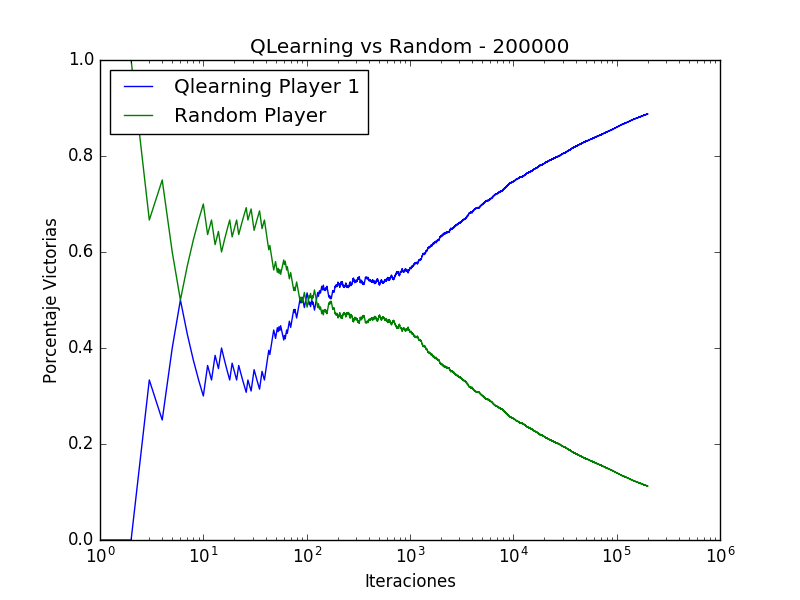
\includegraphics[scale=0.35]{img1/QlearningVsRandom_200000_6x5_hernan.png}
        \caption{Qlearning vs Random 200000 juegos - Set 1}
  \end{minipage}
 \begin{minipage}{.5\textwidth}
	\centering
	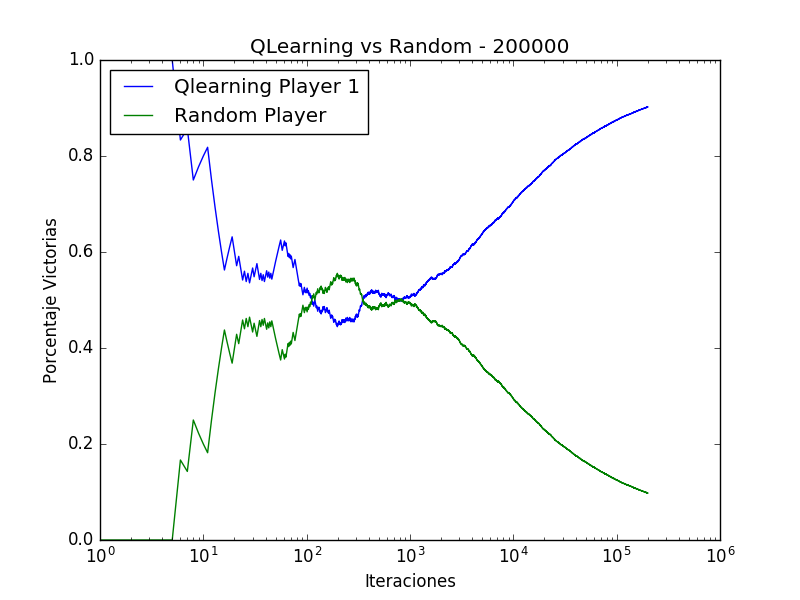
\includegraphics[scale=0.35]{img1/QlearningVsRandom_200000_6x5_cyntia.png}
        \caption{Qlearning vs Random 200000 juegos - Set 2}
  \end{minipage}
\end{figure}


\begin{figure}[H]
 \centering
 \begin{minipage}{.45\textwidth}
  %\begin{minipage}[c]{1\textwidth}
	\centering
	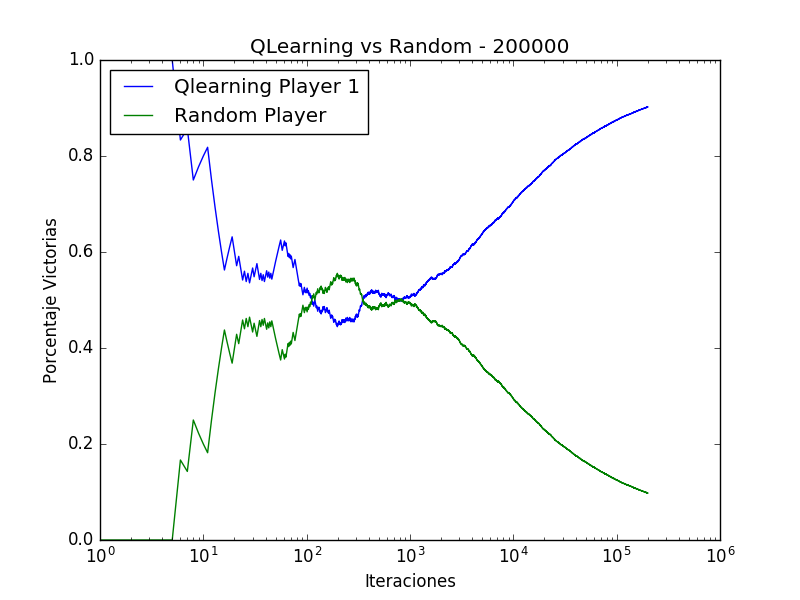
\includegraphics[scale=0.35]{img1/QlearningVsRandom_200000_6x5_cyntia.png}
        \caption{Qlearning vs Random 200000 juegos - Set 3}
  \end{minipage}
\end{figure}


%\begin{frame}
%\begin{figure}[h]
% \centering
%  \begin{minipage}[c]{1\textwidth}
%	\centering
%	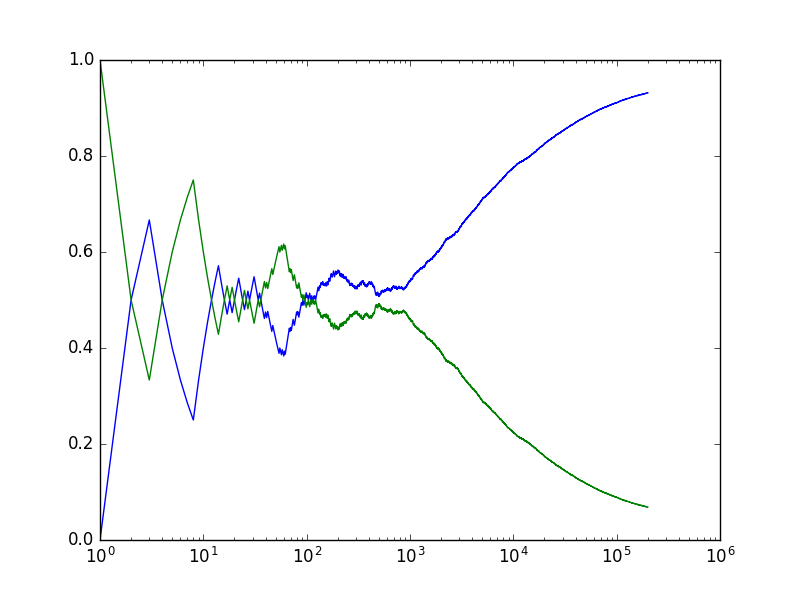
\includegraphics[scale=0.5]{img/QlearningRandomEgreedy200000.png}
%        \caption{Qlearning vs Random 200000 juegos}
%  \end{minipage}
%\end{figure}
%\end{frame}

Observamos que efectivamente el jugador QLearner aprende, pues a medida que aumenta la cantidad de juegos gana mayor cantidad de partidas. Esto no podemos
observarlo en el jugador random.  \\

Otra observación realizada es que en los tres casos, nuestro agente comienza a ganar a partir del orden de $10^{3}$. Por esta razon decidimos testear manualmente que tan bien jugaba,
asi que decidimos jugar contra él para corroborarlo. Al enfrentarlo notamos dos comportamientos interesantes para destacar.

El primer escenario sucedía cuando nuestro agente estaba por perder. Mas especificamente se da cuando es el turno del agente, y el otro jugador tiene dos posibles líneas de tres para completar y ganar.
Es decir, sin importar si el QLearner bloquea alguna de las líneas, el otro jugador ganará en el siguiente turno. La acción que toma el agente era la de ignorar los dos bloques y formar una línea de 2 con el objetivo que, suponemos, si el otro jugador se confunde, en el siguiente paso el agente pueda ganar.

El segundo escenario sucede siempre que el agente juega primero. Para este escenario suponemos que el Qlearner aprendió una estrategia ganadora. Esta es muy parecida a la de que se utiliza en el juego de ta-te-ti de formar una L. El agente juega de tal forma que hace una serie de movimientos que lleva a que sin importar donde ponga la próxima ficha el contrincante, nuestro agente tendrá otras dos posibilidades para ganar.
Para que el lector pueda probar esto y jugar, debe correr el código por default (Ver seccion de instrucciones de uso)

Nos pareció muy llamativo este comportamiento que logró aprender el agente, y lo tomamos como una prueba fehaciente de que el modelo realmente está aprendiendo la naturaleza detrás del juego. Mientras que una persona tardaría bastante tiempo en encontrar la estrategia ganadora, el algoritmo lo encontró simplemente al jugar repetidas veces contra un jugador que juega aleatoriamente.
Esto explicaría por que no empatan, ya que como el jugador que comienza tiene una estrategia ganadora siempre va a ganar nuestro agente cuando le toque comenzar.\\

Lo único que todavía nos llama la atención es el bajo valor que usa de exploración. El resto de los parametros nos parecieron bastante razonables en cuanto a balanceo de utilización de recompensas futuras y actuales, información reciente y futura e inicialización de Q.
Para las pruebas subsiguientes utilizamos el Set 3.\\

Nos preguntamos que pasaría si poníamos a jugar a dos Qlearners. Esperamos ver un comportamiento similar al que tuvo cuando se jugó contra un jugador random, es decir, en algun momento se encuentra la estrategia ganadora y quien comience la partida ganará.\\

A continuación mostramos los resultados de dos jugadores Qlearner para diferente número de iteraciones:

\begin{figure}[H]
 \centering
 \begin{minipage}{.45\textwidth}
  %\begin{minipage}[c]{1\textwidth}
	\centering
	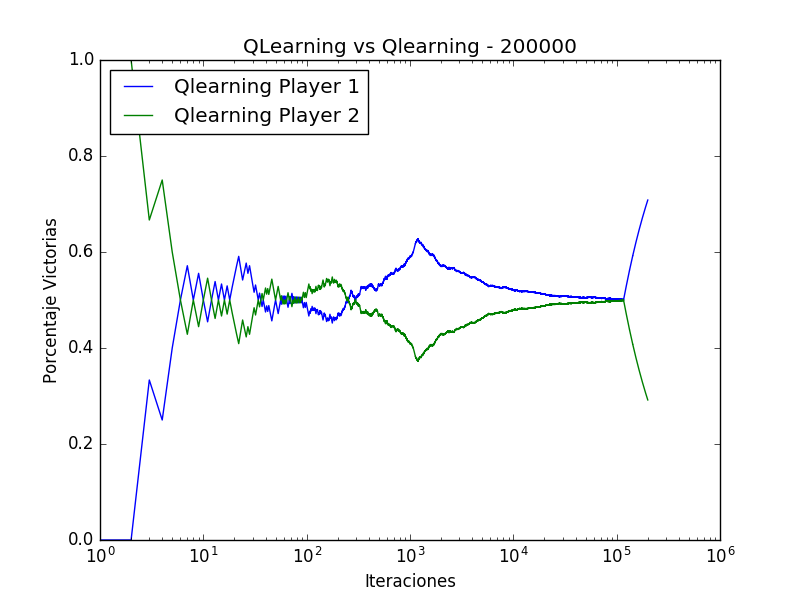
\includegraphics[scale=0.35]{img1/QlearningVsQlearning_200000_6x5_merge.png}
        \caption{Qlearning vs Qlearning 200000 juegos}
  \end{minipage}
 \begin{minipage}{.5\textwidth}
	\centering
	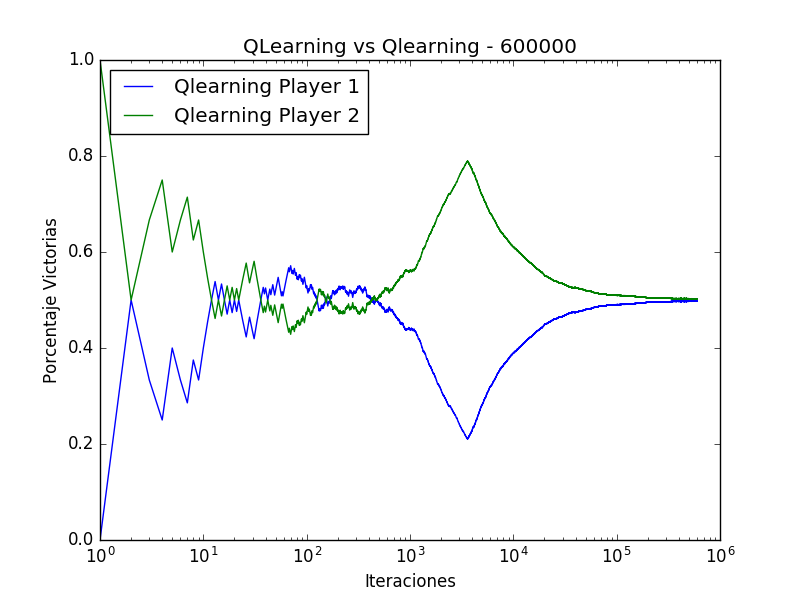
\includegraphics[scale=0.35]{img1/QlearningVsQlearning_600000_6x5_merge.png}
        \caption{Qlearning vs Qlearning 600000 juegos}
  \end{minipage}
\end{figure}


\begin{figure}[H]
 \centering
 \begin{minipage}{.45\textwidth}
  %\begin{minipage}[c]{1\textwidth}
	\centering
	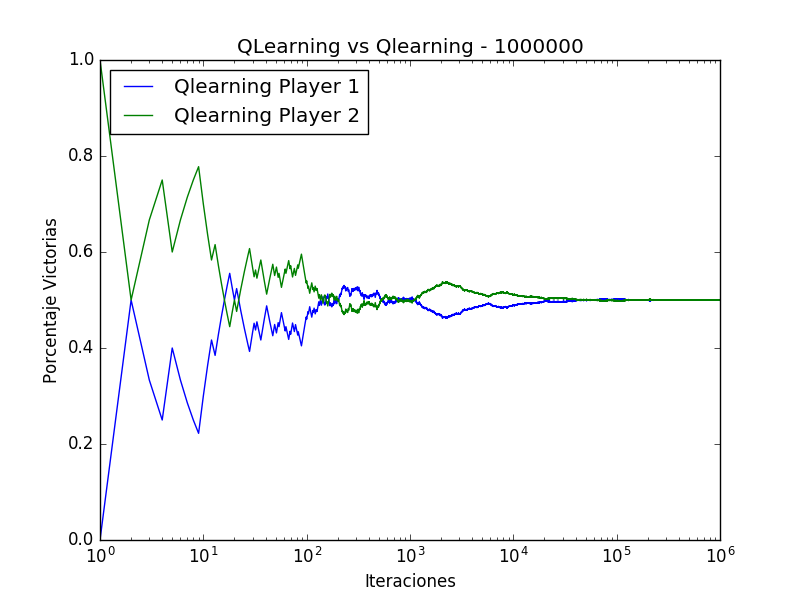
\includegraphics[scale=0.35]{img1/QlearningVsQlearning_1000000_6x5_merge.png}
        \caption{Qlearning vs Qlearning 1000000 juegos}
  \end{minipage}
\end{figure}

Observando los gráficos creímos que pasaba lo mismo que en el caso anterior, es decir que llegado el punto en que se aprendía la estrategia ganadora, quien comienza la partida será el ganador.

Sin embargo, al jugar contra el Qlearner nos encontramos con que no aprendió una estrategia ganadora. Creemos que esto se debe a que al tener un oponente random que realiza jugadas al azar fuerza a que se exploren más opciones de juego con el objetivo de bloquearlo.
Esto explicaría por que al tener un oponente random con un epsilon ``grande'' convierte al juego en ``demasiado'' random, pero si se tiene un oponente Qlearner, tener un epsilon ``bajo'' lo convierte en ``poco'' random. \\

Para tratar de corroborar nuestra hipotesis entrenamos con dos jugadores Qlearners los mismos parámetros que usamos anteriormente pero aumentando el $\epsilon$.
Obteniendo los siguientes resultados:

\begin{figure}[H]
 \centering
 \begin{minipage}{.45\textwidth}
  %\begin{minipage}[c]{1\textwidth}
	\centering
	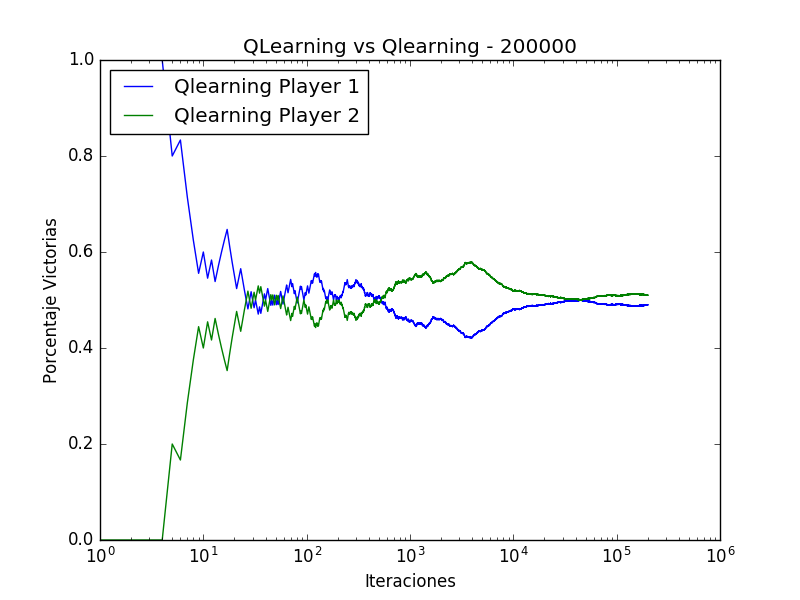
\includegraphics[scale=0.35]{img1/QlearningVsQlearning_200000_6x5_merge_e0p1.png}
        \caption{Qlearning vs Qlearning 200000 juegos - epsilon 1.0}
  \end{minipage}
\end{figure}


Volvimos a jugar contra el jugador entrenado y observamos que ahora si aprendió la estrategia ganadora. Esto explicaría por que inicialmente cuando jugabamos contra un jugador random los mejores parámetros siempre tenían un epsilon bajo, incluso cero.
Lo que todavía no pudimos responder es por que cuando se enfrentan dos Qlearners que no conocen la estrategia ganadora no llegan a empatar. Creemos que tiene que ver con que tener un conjunto grande de estados ganadores, hace que empatar sea dificil y sea mas probable que siempre alguno de los dos gane la partida, incluso no conociendo una estrategia ganadora.\\



\subsection{Experimento 4 en linea en tablero de $7\times6$}
En la sección anterior jugamos con un tablero de dimensión menor a la del juego 4 en linea, es por esto que queremos comprobar si nuestra hipótesis de que si tenemos un buen conjunto de parametros para el tablero mas chico y el juego tres en línea podemos utilizar los mismos para extenderlo al 4 en linea y obtener buenos resultados.

En esta sección experimentamos con el tablero original de $7\times6$, y las reglas originales del 4 en linea, obteniendo los siguientes resultados:\\


%{\large ACA HAY QUE CORRER DE NUEVO ESTO, NO ME MATEN PERO LOS PARAMETROS FINALES
%CUANDO SE JUEGA CONTRA RANDOM SON: \\
%epsilon=0.0001, learning\_rate=0.4, discount=0.9, initialQ=0.0 \\
%Y CUANDO SE JUEGA CONTRA OTRO QLEARNING:
%epsilon=0.1, learning\_rate=0.4, discount=0.9, initialQ=0.0 \\

%HAY QUE CORRER PARA 7x6 4 en linea: \\
%iteraciones 200000 para QLEARNING VS RANDOM
%iteraciones 200000 para QLEARNING VS QLEARNING
%iteraciones 600000 para QLEARNING VS QLEARNING
%iteraciones 1000000 para QLEARNING VS QLEARNING

%SI LA ULTIMA NO ANDA NO PASA NADA.

%}


\begin{figure}[H]
 \centering
  \begin{minipage}[c]{1\textwidth}
	\centering
	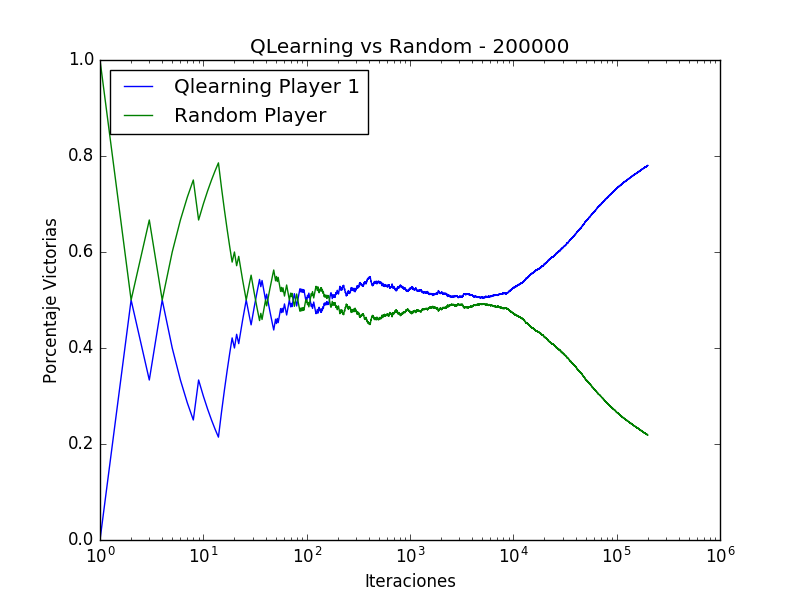
\includegraphics[scale=0.5]{resultados/7x6/QlearningVsRandom_200000_7x6_parametros_informe.png}
        \caption{Qlearning vs Random 200000 juegos}
  \end{minipage}
\end{figure}

Lo que podemos observar del resultado es bastante razonable, como agrandamos el tablero tenemos muchas mas combinaciones, motivo por el cual, tarda mas tiempo en aprender a jugar bien.
Otra observación que notamos al jugar contra el agente entrenado es que este jugaba bastante mal y los resultados fueron bastante pobres. Tampoco fue visible a simple vista una estrategia ganadora tal como pasaba en el tablero mas chico.
Por lo que podemos concluir que nuestro agente no encuentra estrategia ganadora para el caso de $7\times6$ y 4 en línea.


Luego de estos malos resultados decidimos experimentar tal como lo habiamos hecho en el 3 en línea, es decir haciendo que nuestro agente juege contra otro Qlearner. Por lo tanto
experimentamos usando los mismos parametros que contra el jugador random, con la particularidad de que aumentamos el epsilon a 0.1, obteniendo los siguientes resultados:

\begin{figure}[H]
 \centering
 \begin{minipage}{.45\textwidth}
	\centering
	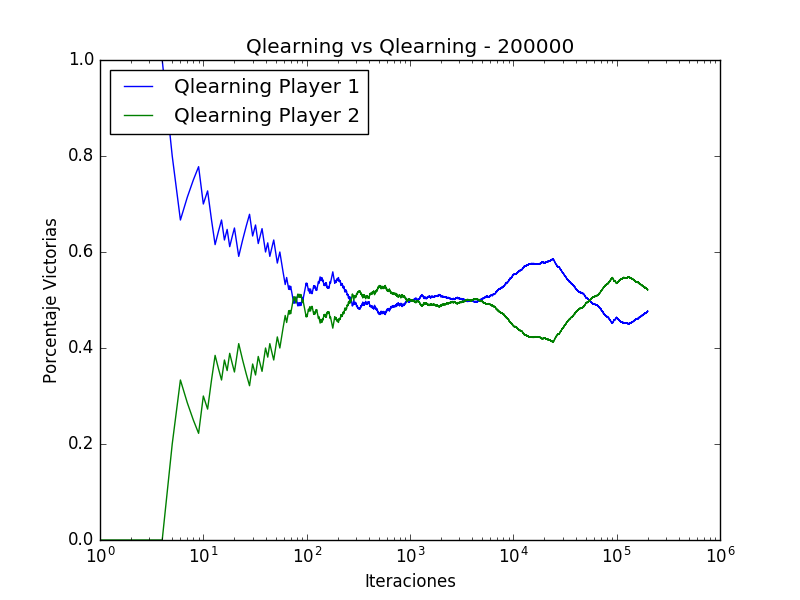
\includegraphics[scale=0.35]{resultados/7x6/QlearningVsQlearning_200000_7x6_parametros_informe.png}
       \caption{Qlearning vs Qlearning 200000 juegos}
  \end{minipage}
 \begin{minipage}{.5\textwidth}
	\centering
	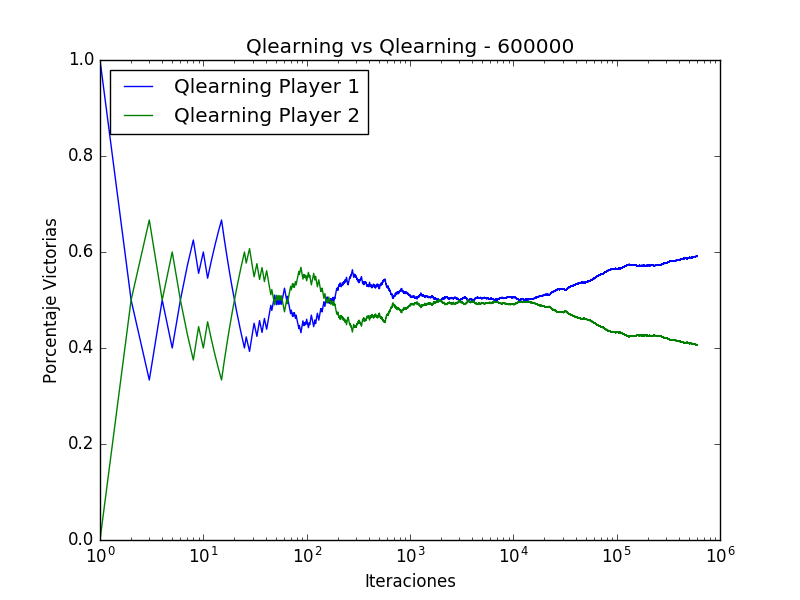
\includegraphics[scale=0.35]{resultados/7x6/QlearningVsQlearning_600000_7x6_parametros_informe.png}
        \caption{Qlearning vs Qlearning 600000 juegos}
  \end{minipage}
\end{figure}

\begin{figure}[H]
 \centering
 \begin{minipage}{.45\textwidth}
  %\begin{minipage}[c]{1\textwidth}
	\centering
	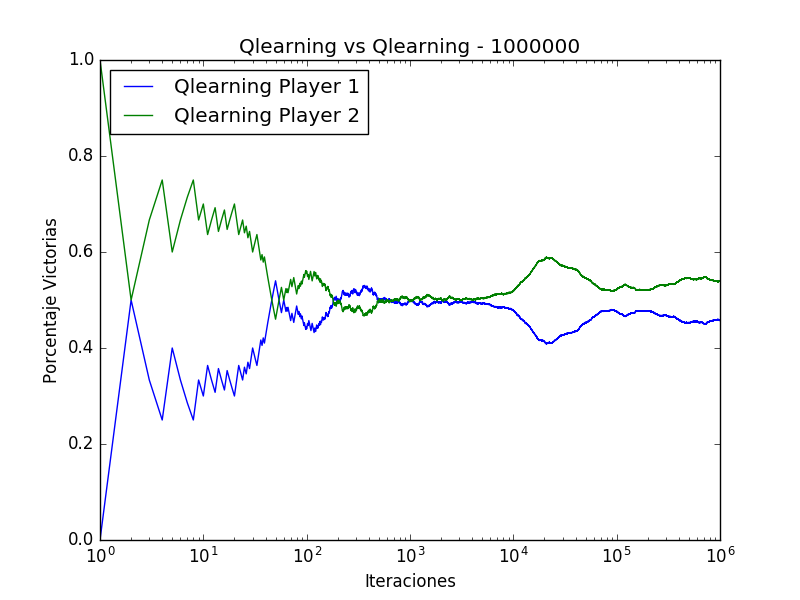
\includegraphics[scale=0.35]{resultados/7x6/QlearningVsQlearning_1000000_7x6_parametros_informe.png}
        \caption{Qlearning vs Qlearning 1000000 juegos}
  \end{minipage}
\end{figure}

Se puede ver una tendencia a estabilizarse en que gana el 50\% de las veces cada jugador, sin embargo, no es del todo claro. En este caso el jugador entrenado tampoco aprende una estrategia ganadora. \\

\todo{FALTA VER QUE PASÓ ACA CON LOS ULTIMOS ENTRENADOS, PUSE ALGO PERO ES INVENTO}


Encontramos que el juego cuatro en línea tiene solución y que con un juego perfecto , el primer jugador puede forzar una victoria, comenzando en la columna central. Por este motivo creemos que sería interesante poder entrenar con muchas mas jugadas y una politica de control como softmax. Que nos ayudaría a ajustar mejor el epsilon a medida que entrenamos. Dejamos estas pruebas en el tintero por cuestiones de tiempo.


%Asi que pensamos en probar otra politica de control: softmax.
%Otra vez necesitamos buscar los parametros. En este caso necesitamos definir un tau y una funcion de decremento ademas de textit{learning rate}, \textit{discount}, cantidad de epocas, y los valores de inicializacion de Q. Para estos ultimos exploramos valores que se encontraban alrededor de los encontrados para la estrategia e-greedy.
%Empezamos con el tabler de 6x5 y 3 fichas y una vez encontrado los parametros pasamos al tablero real.



%{\huge FALTARIA QUE FUNCIONE SOFTMAX Y VER QUE DA.
%LA TEORIA SERIA QUE TIENE QUE SER UN POCO MAS INTELIGENTE PORQUE YA VIMOS QUE LA EXPLORACION LO CAMBIA TODO.
%}\\


%{\huge FALTAN CONCLUSIONES
%}\\


%
% \subsection{Experimento 4 en linea en tablero de $7\times6$}
% En el siguiente experimento decidimos entrenar con el juego completo de 4 en linea, en su formato original de un tablero
% de $7\times6$. Para este caso decidimos experimentar con dos politicas de control: \textit{$\epsilon-greedy$} y
% \textit{softmax}. En ambos casos realizamos 500000 iteraciones de juego, y para cada caso entrenamos a nuestro agente
% contra un jugador random y contra otro agente de Qlearning. \\
% Los parametros utilizados tanto para \textit{$\epsilon-greedy$}, como para \textit{softmax} fueron los obtenidos por la
% estrategia de Grid search previamente explicada.
%
% Los resultados obtenidos en cada caso fueron:
%
% \todo{Poner resultados Qlearn vs Qlearn(epsilon greedy)}
%
% \todo{Poner resultados Qlearn vs Qlearn(softmax)}
%
% \todo{Poner resultados Qlearn vs random(epsilon greedy)}
%
% \todo{Poner resultados Qlearn vs random(softmax)}
%
% \subsection{Experimento 3 en linea en tablero de $6\times5$}
